\subsection{Implementation in SU2}

SU2 is an open-source software suite that is used to solve non-linear Partial Differential Equations (PDE) along with PDE-constrained optimization problems while utilizing unstructured meshes \cite{su21}. The framework is general and meant to be extensible to any sets of governing equations for multi-physics problems. The focus for this work is its Reynolds Averaged Navier-Stokes (RANS) solver capable of simulating compressible, turbulent flows found in aerospace engineering and design problems. To ensure the reliability of the baseline SU2 RANS solver, extensive validation studies of the SU2 platform have been conducted across a diverse assortment of turbulent flows \cite{su22}. 

SU2 is actively developed around the world. It has been released under an open-source license and is freely available to the community, so that developers may contribute to the source code and further improve the accuracy and capabilities of the suite. To accomplish ease of use, the SU2 includes industry-standard solver technology for turbulent flows while also developing numerical solution algorithms that result in robust rates of convergence. Finally, to aid with gradient-based optimization, SU2 includes a discrete adjoint solver implementation for efficiently computing the gradient of any quantity of interest with respect to any design variable.

This section outlines details of the implementation of the eigenspace perturbation methodology into the CFD solver. The first part of the discussion outlines the algorithms, and the steps required to perform the eigenspace perturbation within the CFD solver. The second part focuses on its explicit implementation via computer code and its integration with the SU2 solver. 

\begin{figure}
\centering
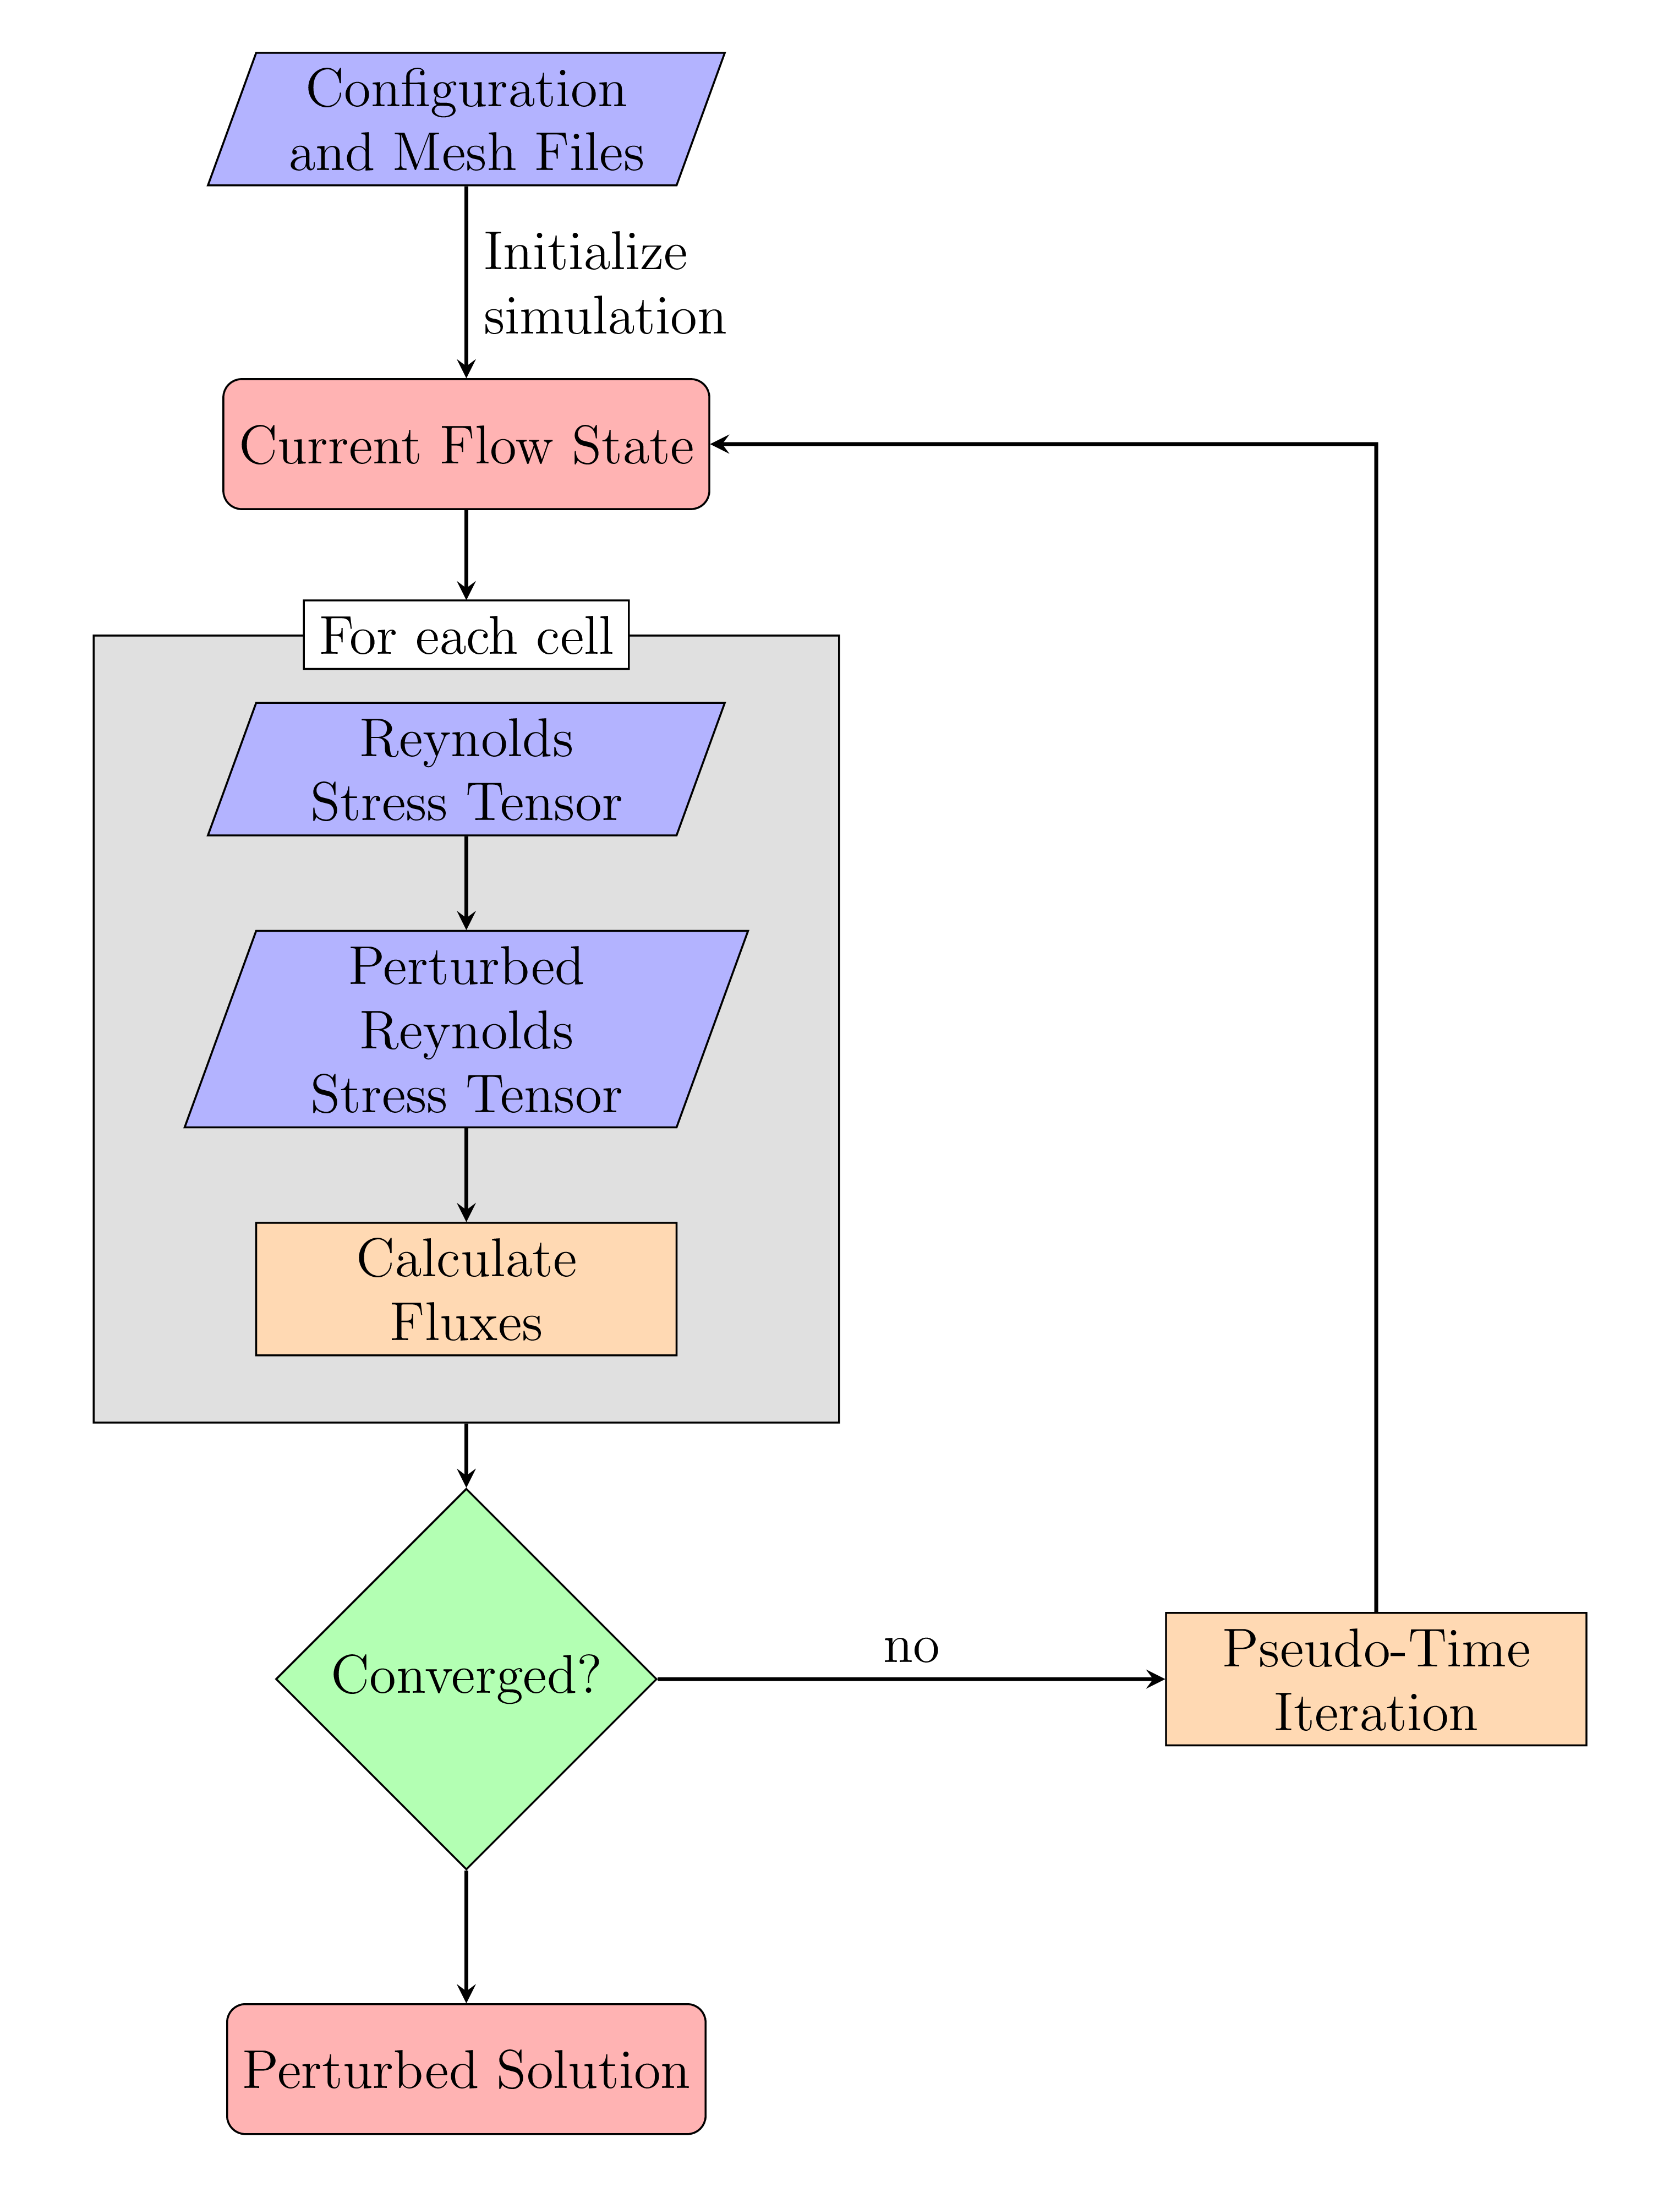
\includegraphics[width=0.75\textwidth]{suthesis/images/su2_implmentation.png}
\caption{Flow chart showing the implementation of EQUiPS within SU2 \label{fig:equips_overview}}
\end{figure}

Fig. \ref{fig:equips_overview} shows where the eigenspace perturbation fits within the context of the CFD solver. The perturbation is carried out for each cell at each pseudo-time step. This process in repeated until the flow simulation converges and outputs a perturbed solution. 

\begin{figure}
\centering
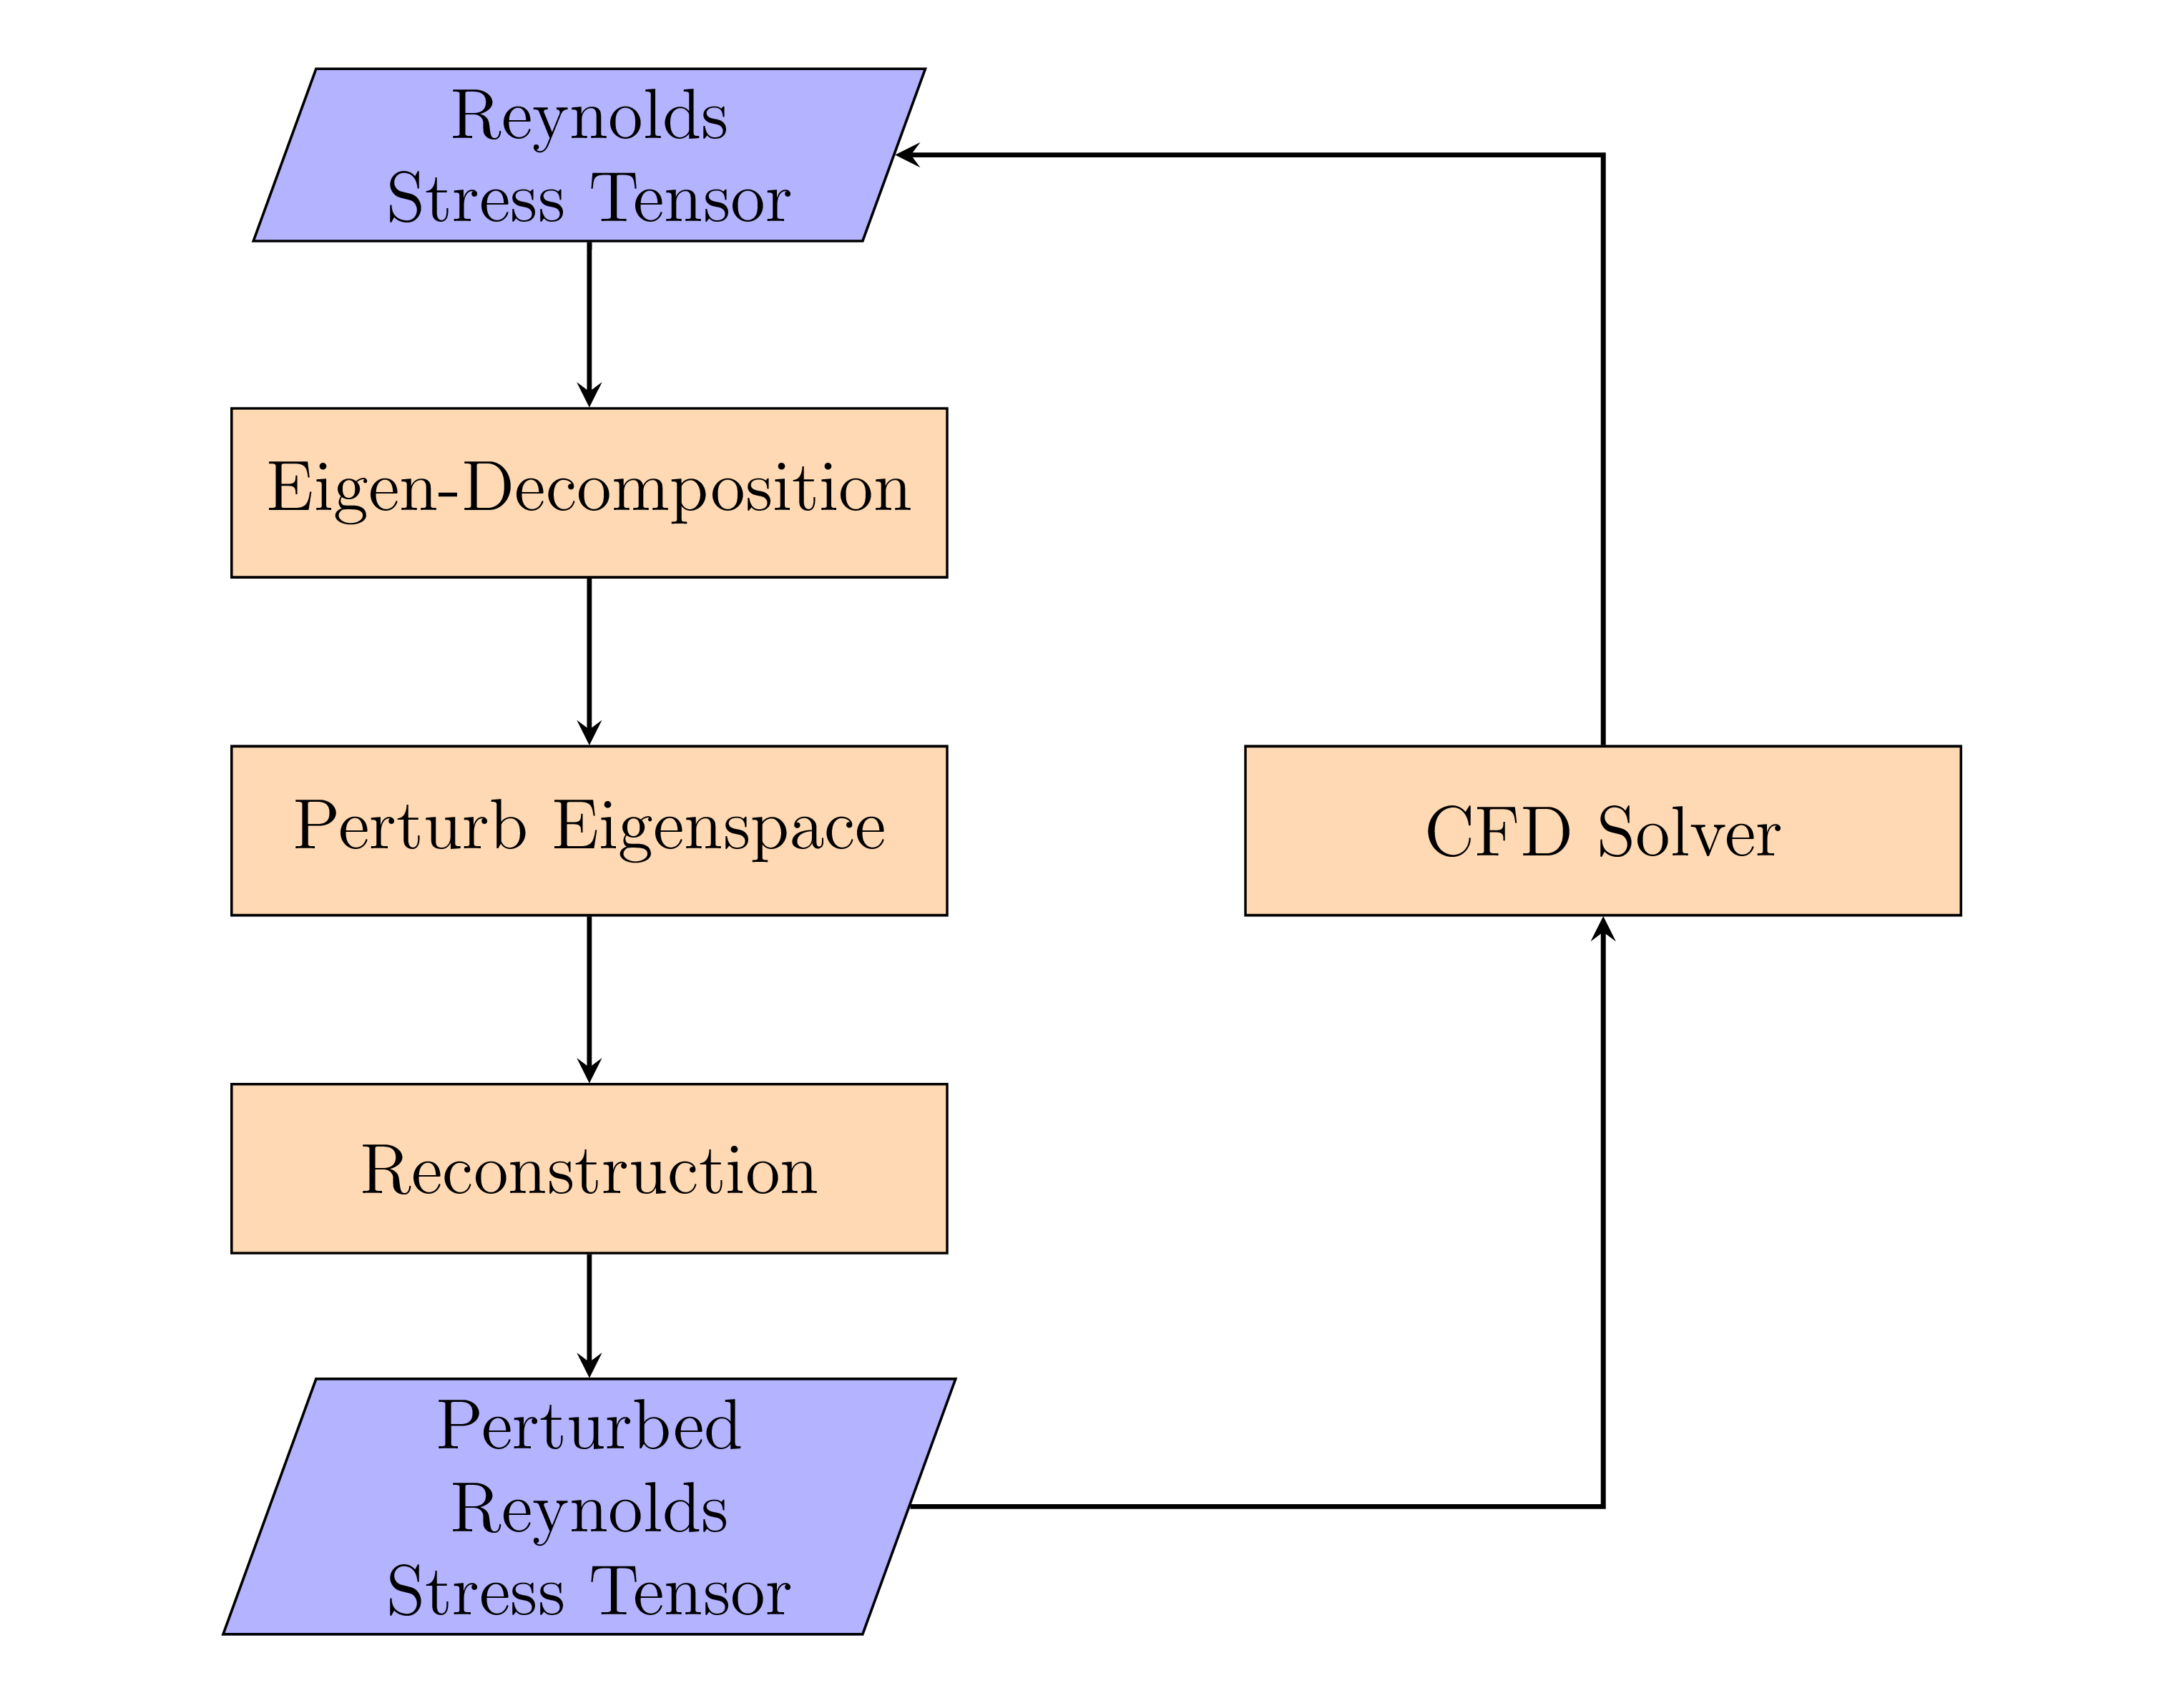
\includegraphics[width=0.75\textwidth]{suthesis/images/eigenspace_pert.png}
\caption{Schematic outlining interaction between CFD solver and perturbation methodology, at each cell and iteration.\label{fig:perturbation_schematic}}
\end{figure}

Fig. \ref{fig:perturbation_schematic} focuses on the steps required to perform the eigenspace perturbation. The first step is to use the flow field to calculate the Reynolds stress tensor, using Equation \ref{equ:rst}, at each cell in the computational domain. The anisotropic part of the tensor, $b_{ij}$ in Equation \ref{equ:rst_decomp}, is decomposed into its eigenvalues and eigenvectors, as shown in Equation \ref{equ:eigendecomposition}. To do this efficiently, the anisotropic tensor's symmetry is leveraged. First, the symmetric tensor is reduced to a symmetric tridiagonal form using the Householder's transform and accumulating orthogonal similarity transformations. This is based on the TRED2 procedure outlined by \cite{tred2a}. Details of the application of the routine can be found in \cite{numres}. Then, the eigenvalues and eigenvectors of this symmetric tridiagonal matrix are computed and sorted using the TQL2 procedure outlined in \cite{tred2b}. These two steps provide a complete eigen-decomposition of the Reynolds stress tensor at a cell in the domain.

The eigenvalues are used to project the stress state onto the barycentric anisotropy invariant map using Equation \ref{equ:barycentric_mapping}. According to the specific perturbation that is being performed, the stress state, denoted by the coordinates $\mathbf{x}$, is perturbed towards one of the vertices of the barycentric map. An under-relaxation factor is used to ensure solution stability. For example, if the stress state is being perturbed towards the 1-component state, the perturbed stress state is represented by the coordinates, 
\begin{equation}
    \mathbf{x^*} = \mathbf{x} + r\left ( \mathbf{x}_{1C} - \mathbf{x} \right )
\end{equation}
where $r$ is the under-relaxation factor. This is a user-tunable parameter, but a default value of $r=0.1$ was used for all the results shown in this thesis. 

Using the barycentric coordinates of the perturbed stress stress, $\mathbf{x^*}$, Equation \ref{equ:barycentric_mapping} can be refactored to get the perturbed eigenvalues. This results in 2 equations, one for each coordinate, with three unknown eigenvalues. The fact that the anisotropy tensor has a zero trace i.e. 
\begin{equation}
    \lambda_1 + \lambda_2 + \lambda_3 = 0
\end{equation}
provides the third equation required to solve the system of equations for the perturbed eigenvalues.

Similarly, for the eigenvector perturbation, the eigenvectors of the Reynolds stress tensor at a cell are permuted to $v_{min}$ or $v_{max}$, depending on the specific perturbation that is being performed.  After this step, the Reynolds stress tensor at each cell is reconstructed from these perturbed eigenvalues and eigenvectors. Additionally, dependent quantities like the turbulence production tensor are re-constituted using this perturbed Reynolds stress tensor. These are input back into the CFD solver for the next iteration. This process continues till numerical convergence as determined by the convergence criteria. 

Focusing on the explicit implementation in SU2, SU2's modular architecture enables integration of this framework without significant alterations to the main code. The module is broken up into two parts: a high-level Python script that sequentially specifies the perturbation to be performed, and C++ code that is added to the existing code base that performs the perturbations during the execution of simulations. For smooth operation, it is best to have performed a baseline simulation with SU2 and have achieved sufficient convergence. This ensures that the mesh file, and the input configuration file are well posed, and, if run through the Python script, can provide converged perturbed solutions.

The Python script takes an input configuration file and a mesh file that are identical to ones that would be used to run the baseline CFD simulation in SU2. The script sets the necessary configuration options to run the EQUiPS framework. These include the direction of the eigenvalue perturbation (aligned towards one of the $1C, 2C$ or $3C$ state on the barycentric triangle for a specific simulation), the magnitude of the eigenvalue perturbation ($\Delta_{B} \in [0,1]$) and the perturbed alignment of the Reynolds stress eigenvector ($v_{min}$ or $v_{max}$, as detailed earlier in this section).  It sequentially runs through the simulations corresponding to perturbed states, creating a new directory for each new simulation, and outputting the results in the respective directories. These results, in conjunction with the previously run baseline solution, can be post-processed to provide the necessary model form uncertainty information. 

The implementation within the existing code base is limited to the two areas where the perturbations are injected into the simulation: in the viscous flux calculations, and in the turbulent flux calculations. The perturbed stress tensors are used to calculate the viscous and turbulent fluxes to advance each node to the next pseudo-timestep. In the case of the SST turbulence model \cite{sst}, the effects of the eigenvector perturbation manifests itself in the turbulence production term. 

The new perturbed fluxes are then used to march the solution forward in pseudo time. As the solution converges, the Reynolds Stress also converges to its perturbed state. Once a perturbed solution is converged, the Python script moves on to the next eigenspace perturbation to be performed. It creates a new directory and a new configuration file to specify the perturbation to be performed. This continues until all the specified perturbed simulations are complete. 

In the spirit of \textit{versatility}, the implementation was developed with the aim of reducing the number of user-defined inputs as much as possible. This allows the framework to be used without in-depth knowledge of the mechanics behind it. The details of the perturbations (componentality, eigenvector permutation etc.) are abstracted away to provide a clean user interface that does not deviate from the work flow of running a regular CFD simulation. For the potential expert user, all the options used for the module can also be specified in the configuration file, without the need for the Python script. 